\documentclass[preprint,12pt]{elsarticle}

% Basic packages
\usepackage[a4paper, margin=1in]{geometry}
\usepackage{graphicx}
\usepackage{amsmath}
\usepackage{hyperref}
\usepackage{longtable}
\usepackage{booktabs}
\usepackage{multirow}
\usepackage{pdflscape}
\usepackage{caption}
\captionsetup[table]{skip=10pt}

% Add Unicode support
\usepackage[utf8]{inputenc}
\usepackage[T1]{fontenc}
\usepackage{textcomp}

% Add color support
\usepackage{xcolor}
\newcommand{\sm}[1]{\textcolor{blue}{#1}}
\newcommand{\SM}[1]{\textcolor{blue}{#1}}
\newcommand{\jl}[1]{\textcolor{red}{#1}}
\newcommand{\JL}[1]{\textcolor{red}{#1}}

% Line numbering
\usepackage{lineno}
\leftlinenumbers
\renewcommand\linenumberfont{\normalfont\small\color{gray}}

% Add support for text formatting
\usepackage{array}
\usepackage{enumitem}
\usepackage{float}

% Add support for special characters
\usepackage{textcomp}
\usepackage{gensymb}

% Citas en texto tipo APA (p.ej., \citep{key} -> (Gonzales et al., 2023))
\biboptions{authoryear,round,semicolon}

%-----------------------------------------------
% METADATA
\title{Turning spectra into images improves plant trait retrieval with 2D-CNNs}

\author[1,2,3]{Javier Lopatin\corref{cor1}}
\ead{javier.lopatin@uai.cl}

\author[1]{Sebastián Moreno}
\ead{sebastian.moreno@uai.cl}

%\author[2,5]{Dylan Craven}
%\ead{dylan.craven@umayor.cl}

\address[1]{Faculty of Engineering and Science, Adolfo Ibáñez University, Av. Diagonal Las Torres 2460, Santiago, Chile, 7941169}

\address[2]{Data Observatory Foundation, ANID Technology Center No. DO210001, Santiago, Chile, 7510277}

\address[3]{Center for Climate Resilience Research (CR)2, University of Chile, Santiago, Chile, 8370449}

% AGREGAR CORRESPONDING AUTHOR CON COR1
\cortext[cor1]{Corresponding author; javier.lopatin@uai.cl}

%-----------------------------------------------
\begin{document}
\begin{frontmatter}

\end{frontmatter}

\linenumbers

% Prefix all table and figure numbers with "S"
\renewcommand{\thetable}{S\arabic{table}}
\renewcommand{\thefigure}{S\arabic{figure}}

% AGREGAR SECCIONES DE PAPER ACA
\section*{Supplementary Data}

\begin{figure}[htbp]
    \centering
    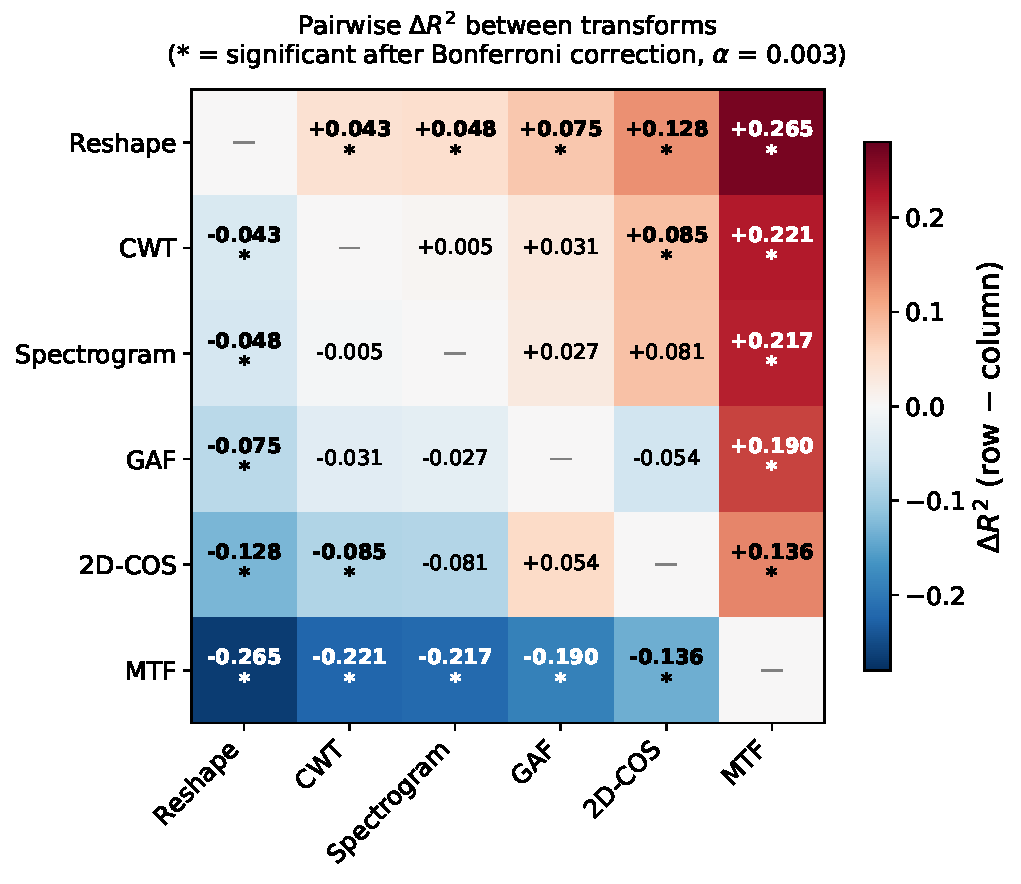
\includegraphics[width=0.75\textwidth]{figures/pairwise_heatmap.pdf}
    \caption{Pairwise differences in mean $R^2$ between 1D-to-2D spectral transformations on the GreenHyperSpectra dataset. Each cell shows $\Delta R^2$ = row $-$ column, computed from paired $t$-tests across 24 observations (8 traits $\times$ 3 seeds). Asterisks (*) denote statistically significant differences after Bonferroni correction ($\alpha = 0.05/15 = 0.003$). Blue indicates the row transform outperforms the column; red indicates the opposite.}
    \label{fig:pairwise_heatmap}
\end{figure}

\begin{figure}[htbp]
    \centering
    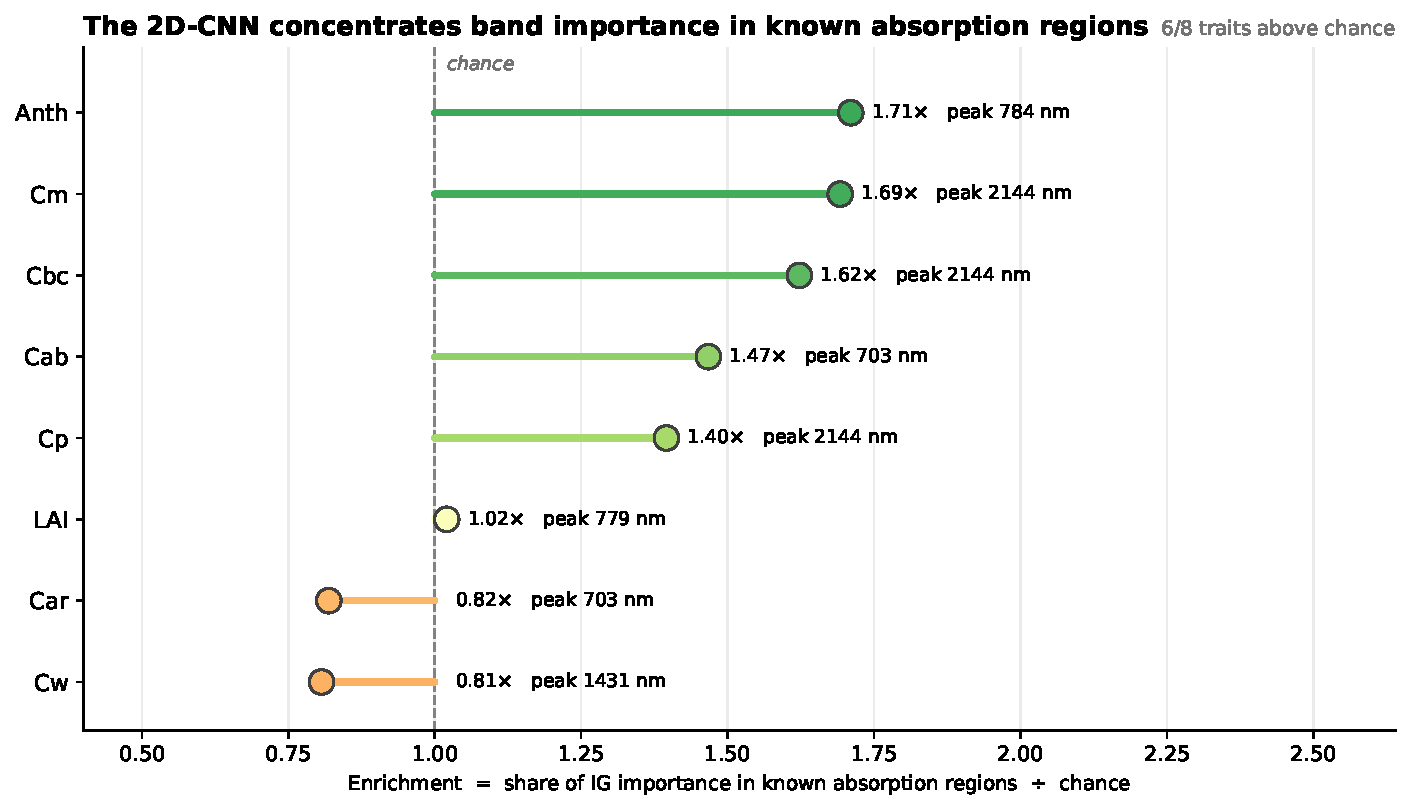
\includegraphics[width=0.85\textwidth]{figures/fig_enrichment.pdf}
    \caption{\jl{Per-trait enrichment of Integrated Gradients importance in known absorption regions. Enrichment is the share of IG importance inside known absorption regions divided by chance. Values above one indicate concentration beyond chance.}}
    \label{fig:enrichment}
\end{figure}

\begin{figure}[htbp]
    \centering
    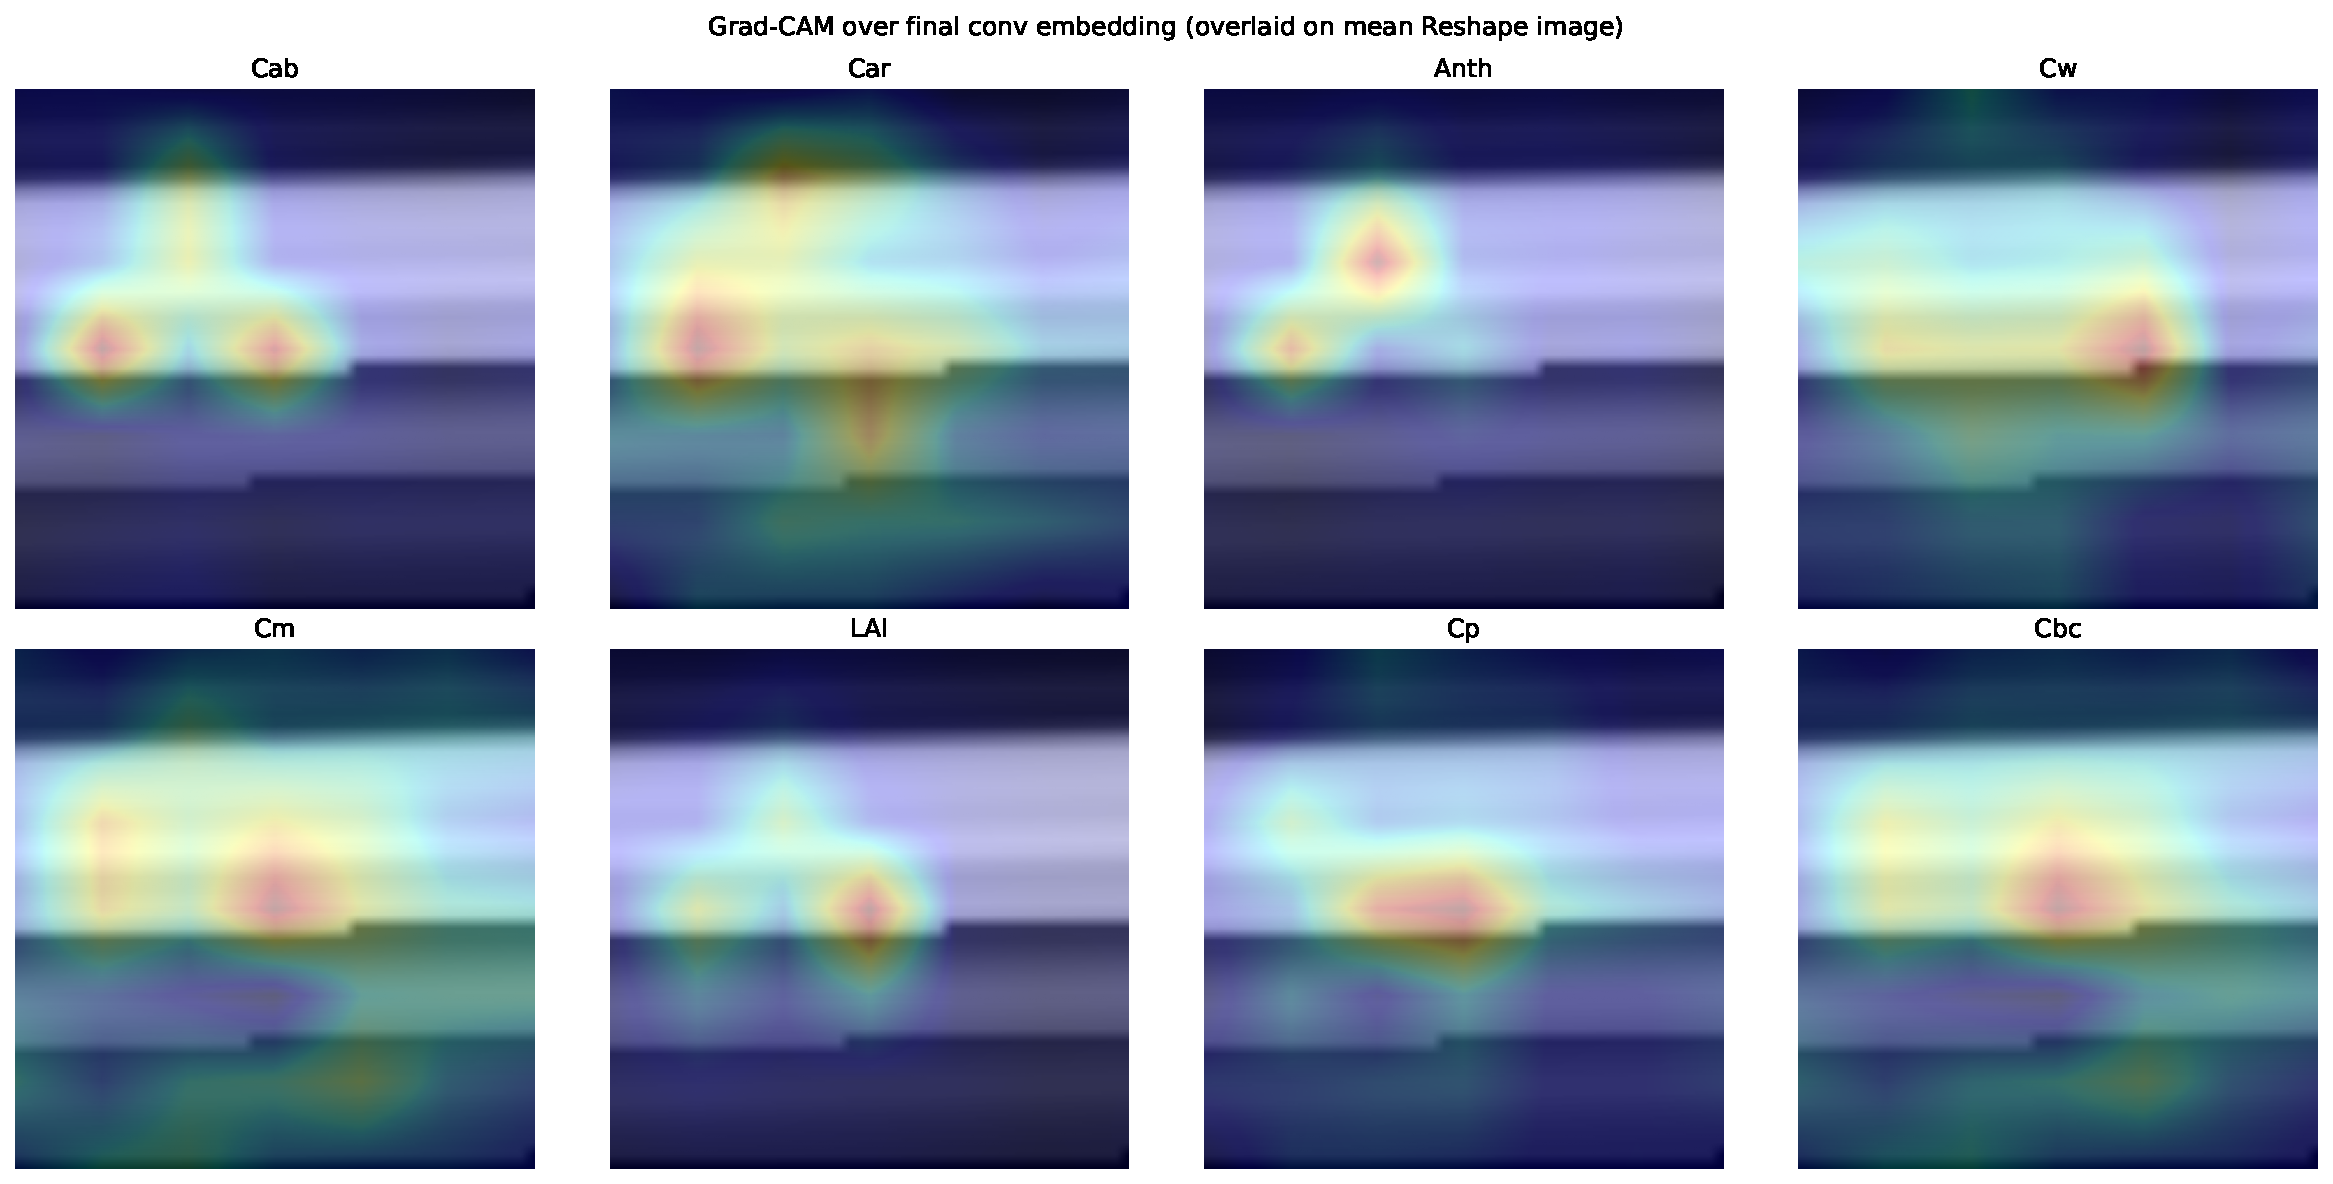
\includegraphics[width=\textwidth]{figures/fig_gradcam_2d.pdf}
    \caption{\jl{Grad-CAM relevance maps on the Reshape image for the eight traits. Warmer colours indicate higher relevance for the predicted trait.}}
    \label{fig:gradcam_2d}
\end{figure}

\jl{Figures~\ref{fig:linking_car} to~\ref{fig:linking_cbc} link the 2D Grad-CAM map and the unfolded 1D importance profile for the remaining seven traits.}

\begin{figure}[htbp]
    \centering
    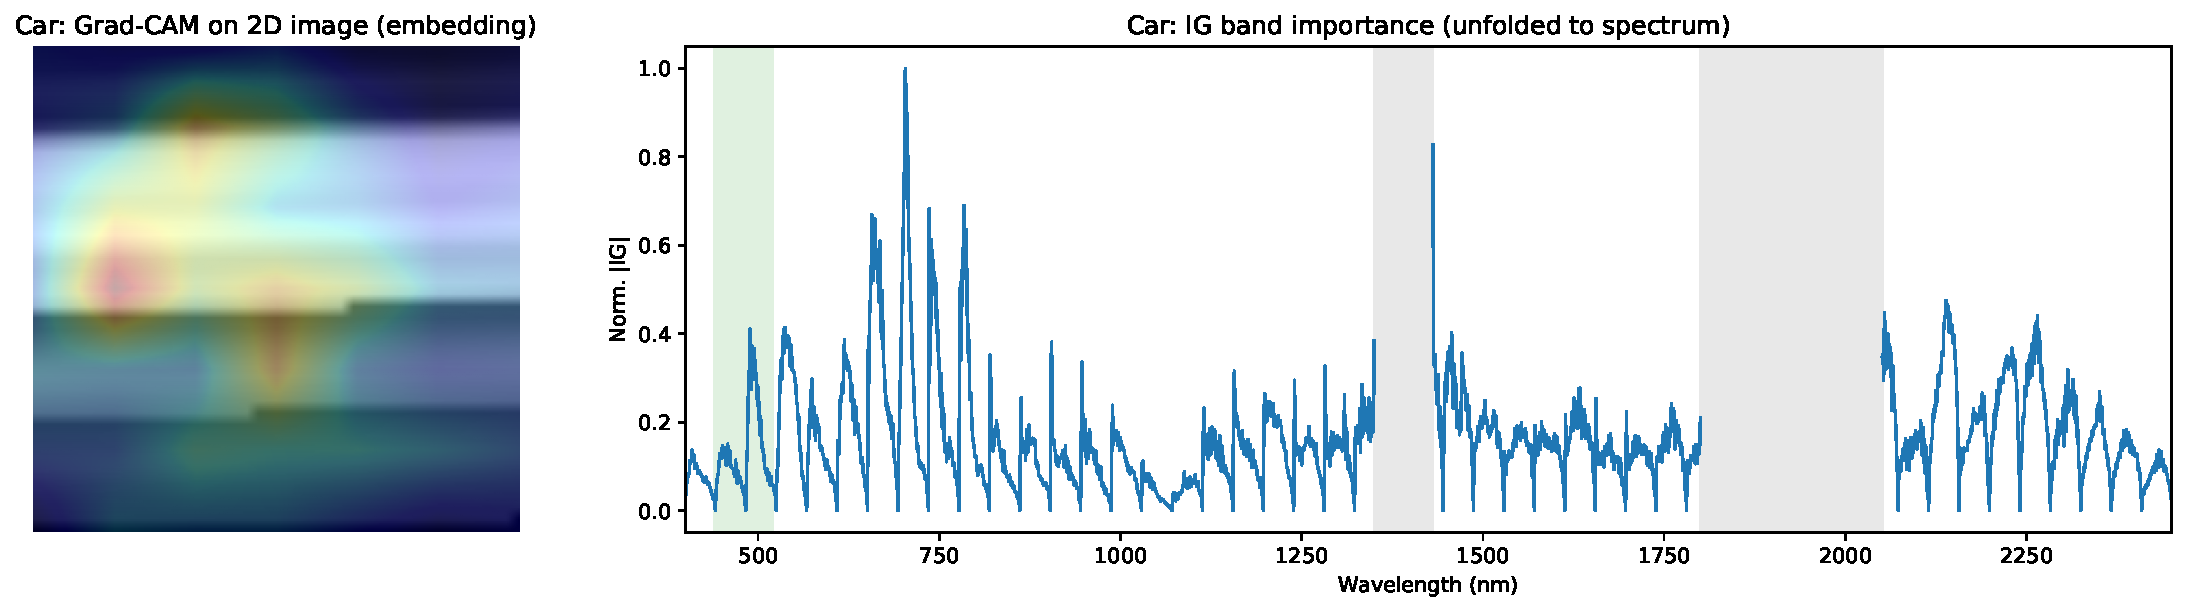
\includegraphics[width=\textwidth]{figures/fig_linking_Car.pdf}
    \caption{\jl{Linking 2D and 1D attribution for carotenoids (C\textsubscript{ar}).}}
    \label{fig:linking_car}
\end{figure}

\begin{figure}[htbp]
    \centering
    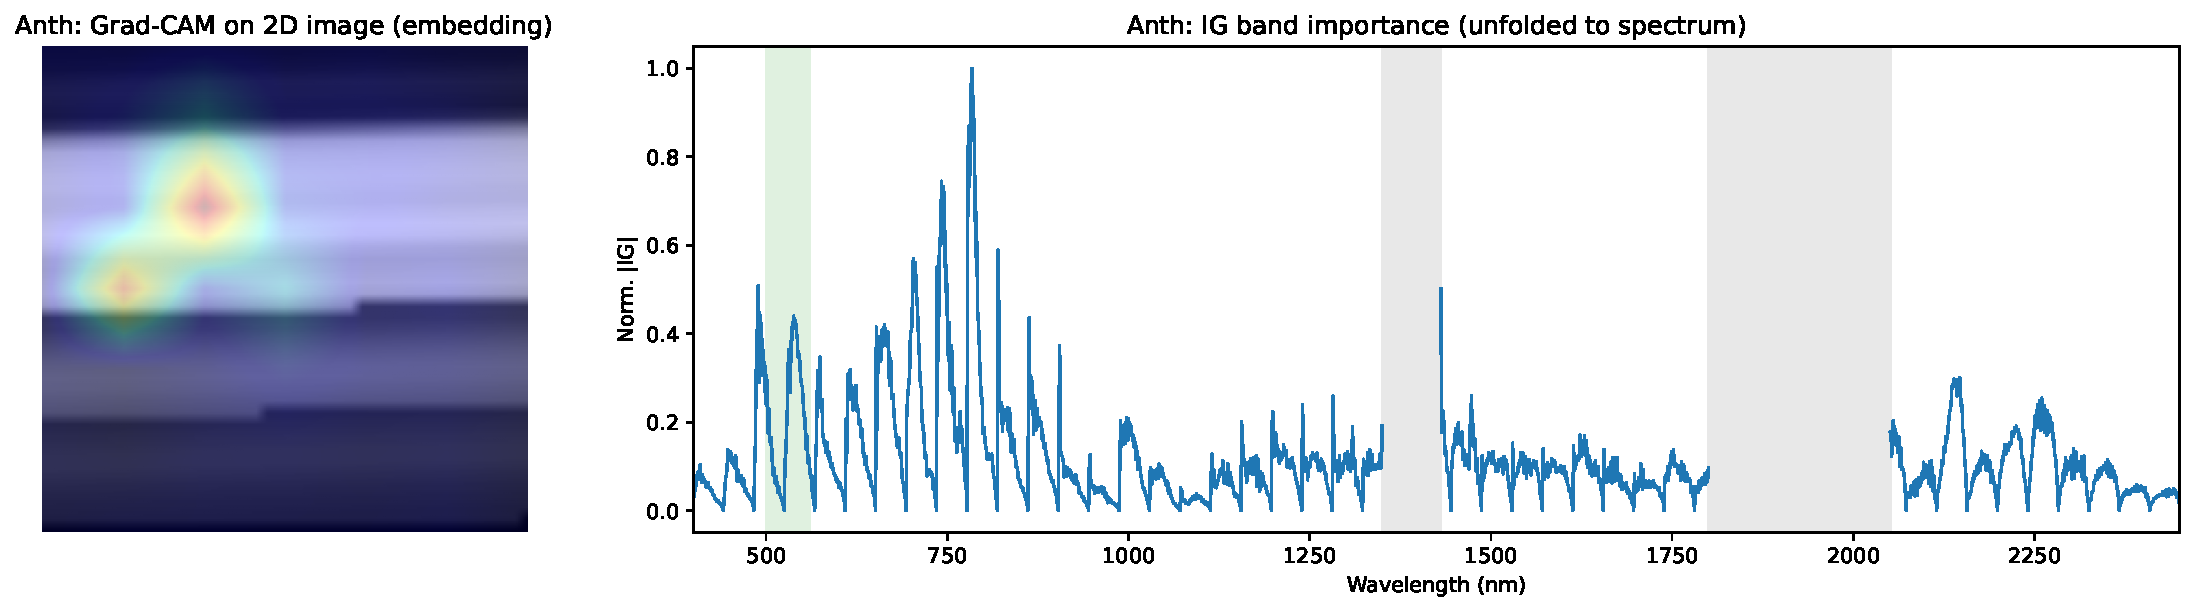
\includegraphics[width=\textwidth]{figures/fig_linking_Anth.pdf}
    \caption{\jl{Linking 2D and 1D attribution for anthocyanins (C\textsubscript{anth}).}}
    \label{fig:linking_anth}
\end{figure}

\begin{figure}[htbp]
    \centering
    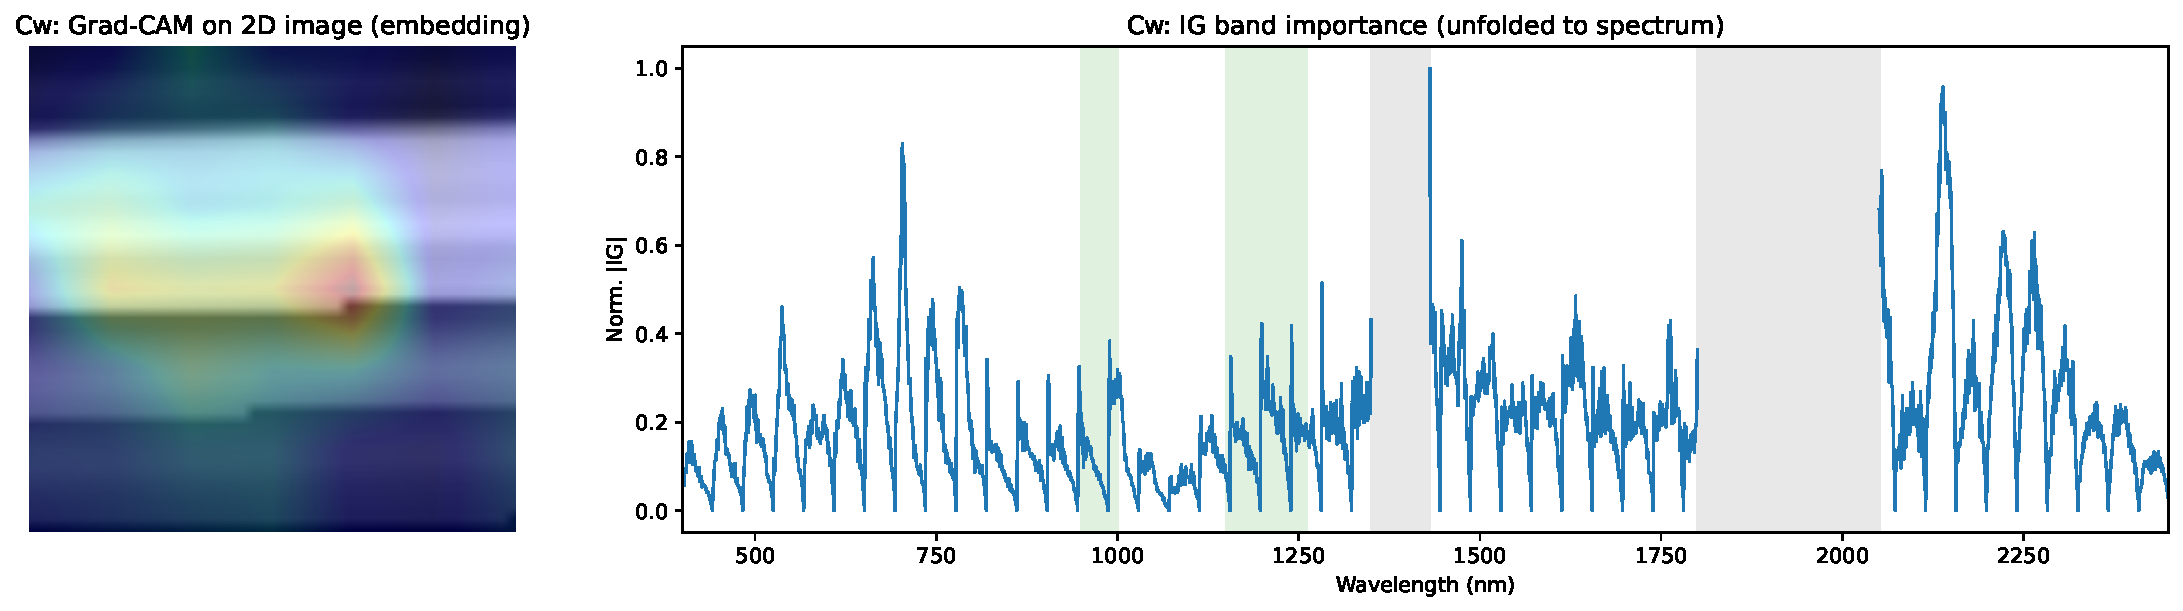
\includegraphics[width=\textwidth]{figures/fig_linking_Cw.pdf}
    \caption{\jl{Linking 2D and 1D attribution for equivalent water thickness (C\textsubscript{w}).}}
    \label{fig:linking_cw}
\end{figure}

\begin{figure}[htbp]
    \centering
    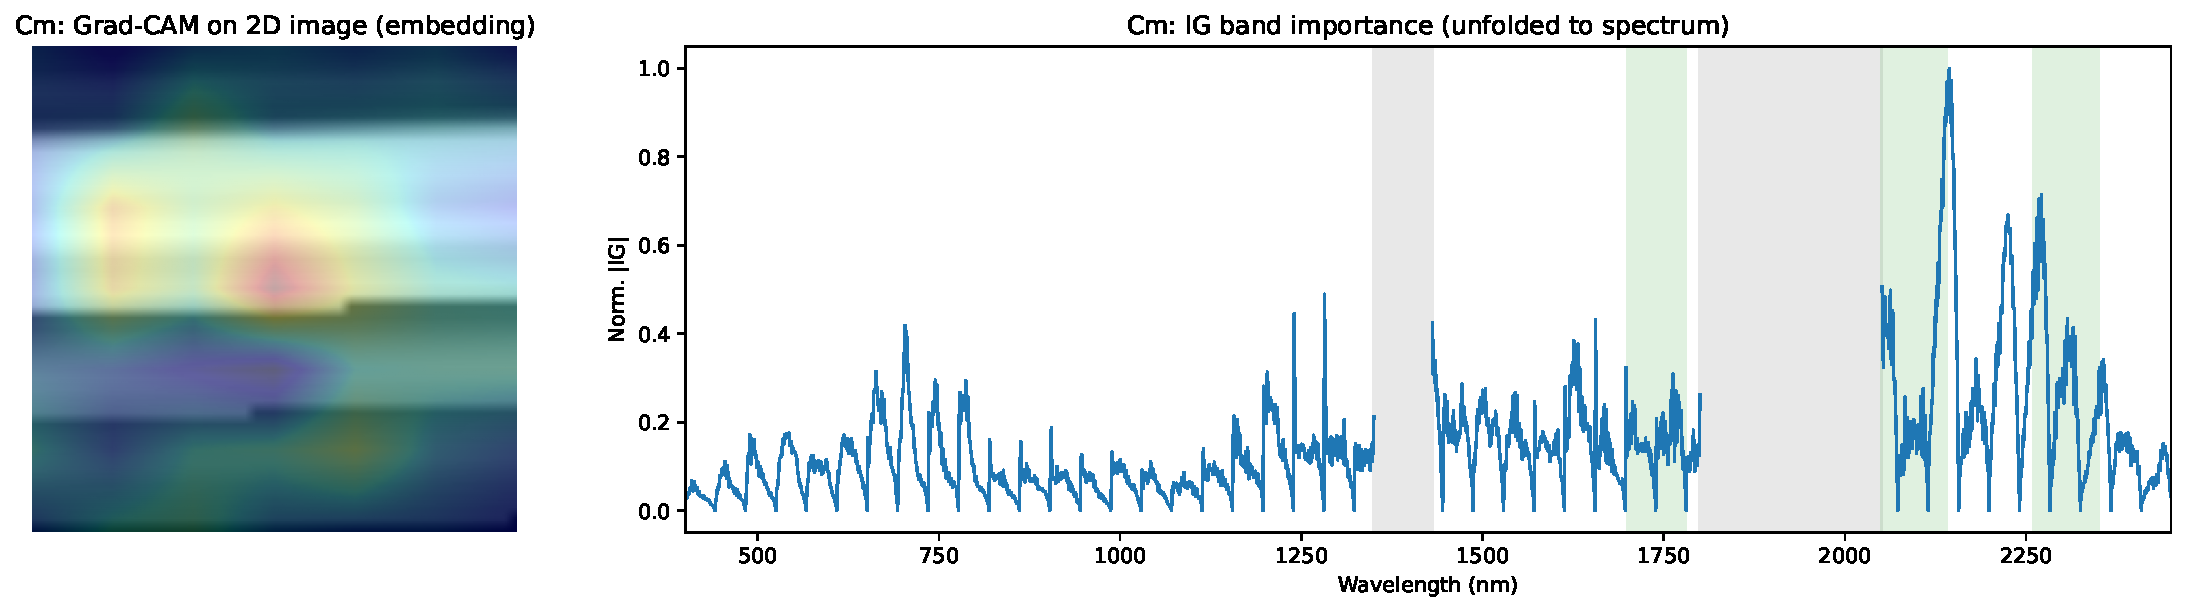
\includegraphics[width=\textwidth]{figures/fig_linking_Cm.pdf}
    \caption{\jl{Linking 2D and 1D attribution for leaf mass per area (C\textsubscript{m}).}}
    \label{fig:linking_cm}
\end{figure}

\begin{figure}[htbp]
    \centering
    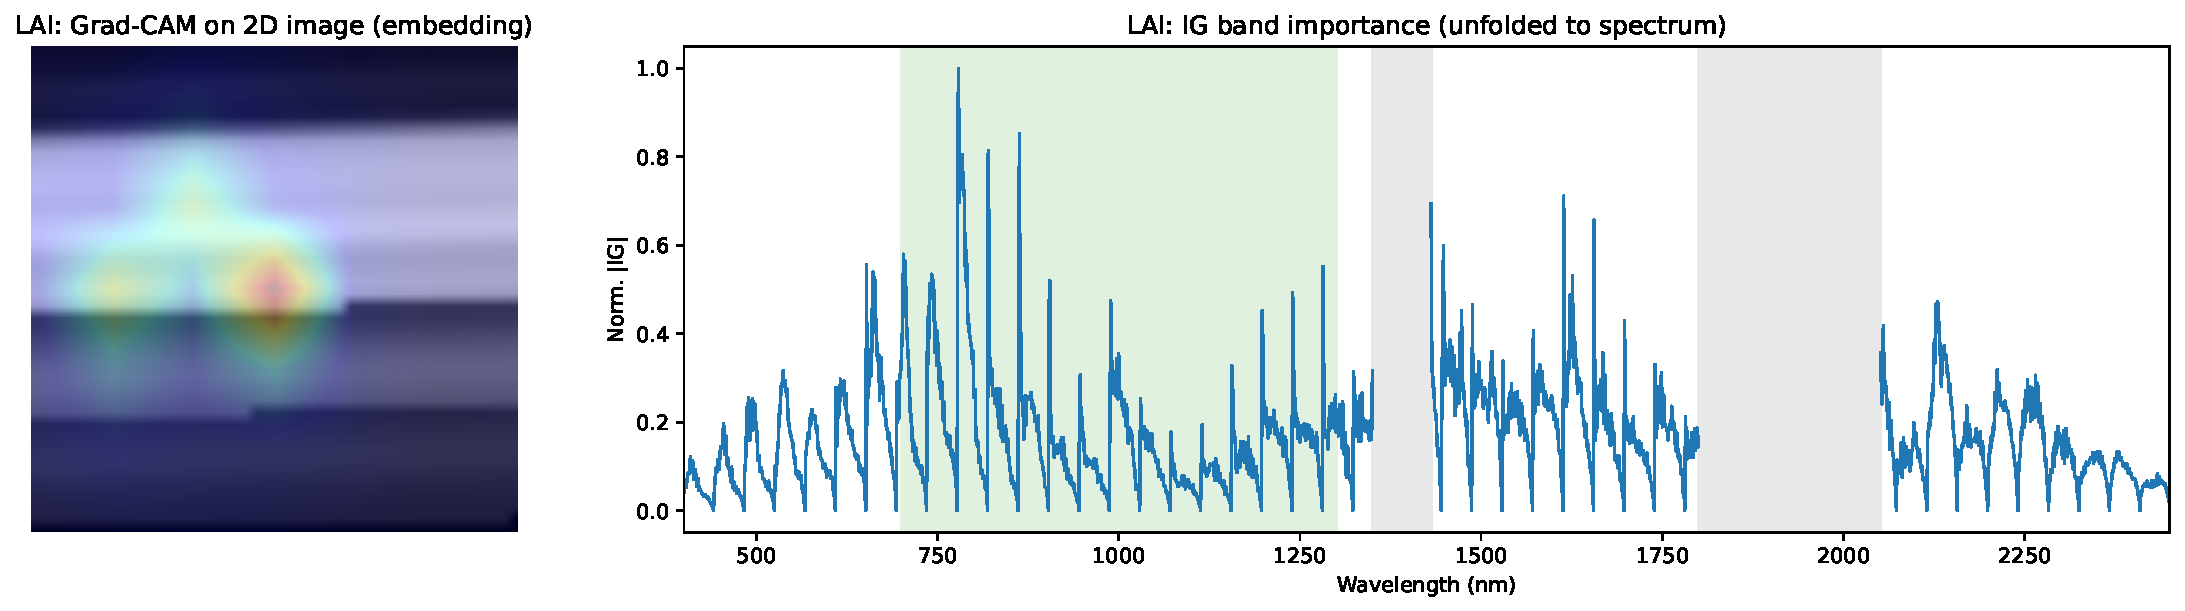
\includegraphics[width=\textwidth]{figures/fig_linking_LAI.pdf}
    \caption{\jl{Linking 2D and 1D attribution for leaf area index (LAI).}}
    \label{fig:linking_lai}
\end{figure}

\begin{figure}[htbp]
    \centering
    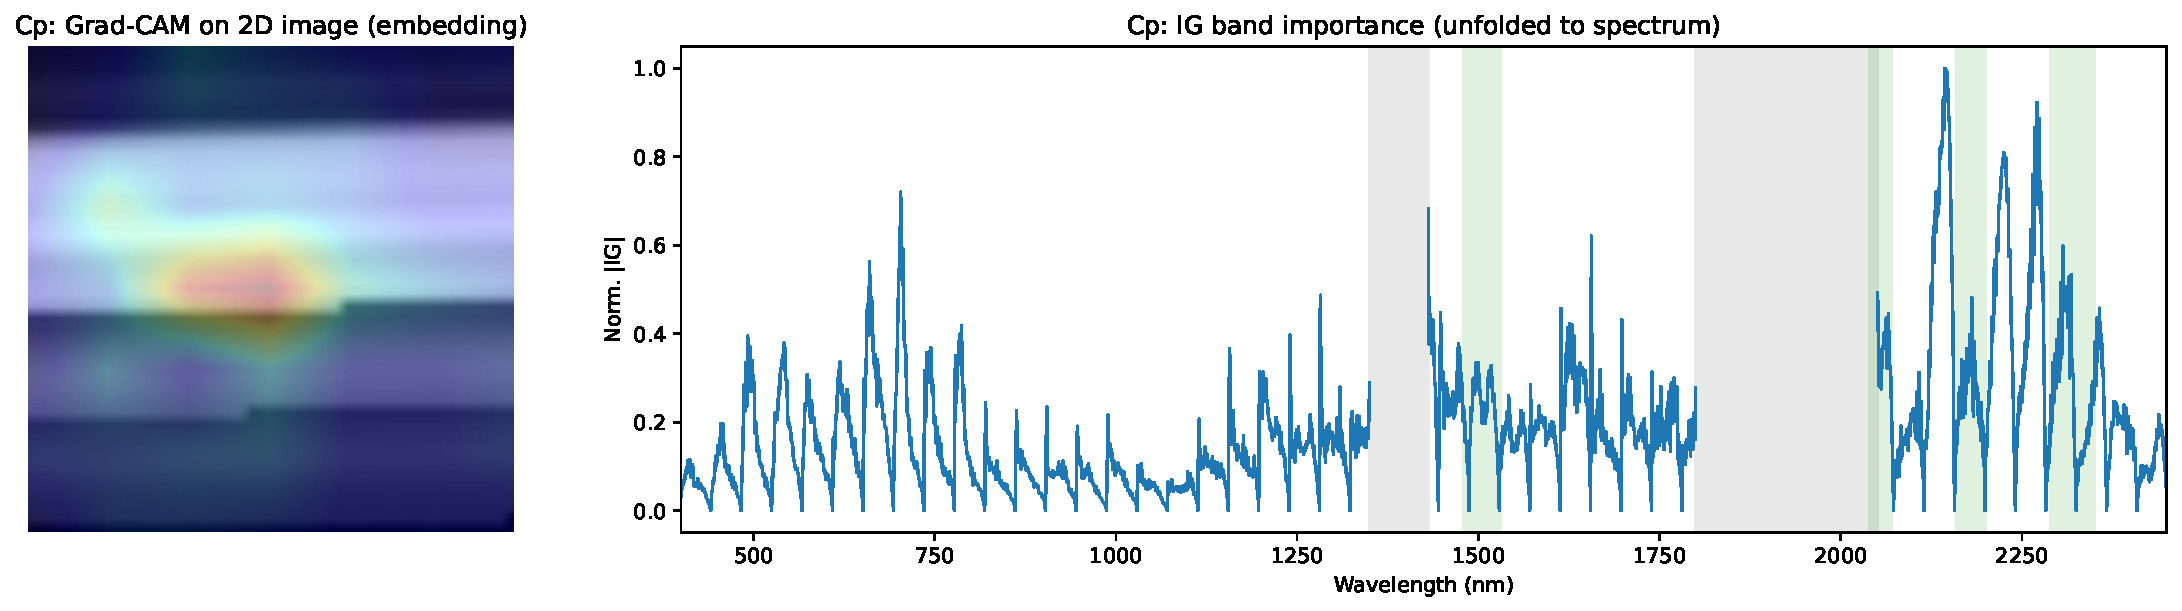
\includegraphics[width=\textwidth]{figures/fig_linking_Cp.pdf}
    \caption{\jl{Linking 2D and 1D attribution for protein content (C\textsubscript{p}).}}
    \label{fig:linking_cp}
\end{figure}

\begin{figure}[htbp]
    \centering
    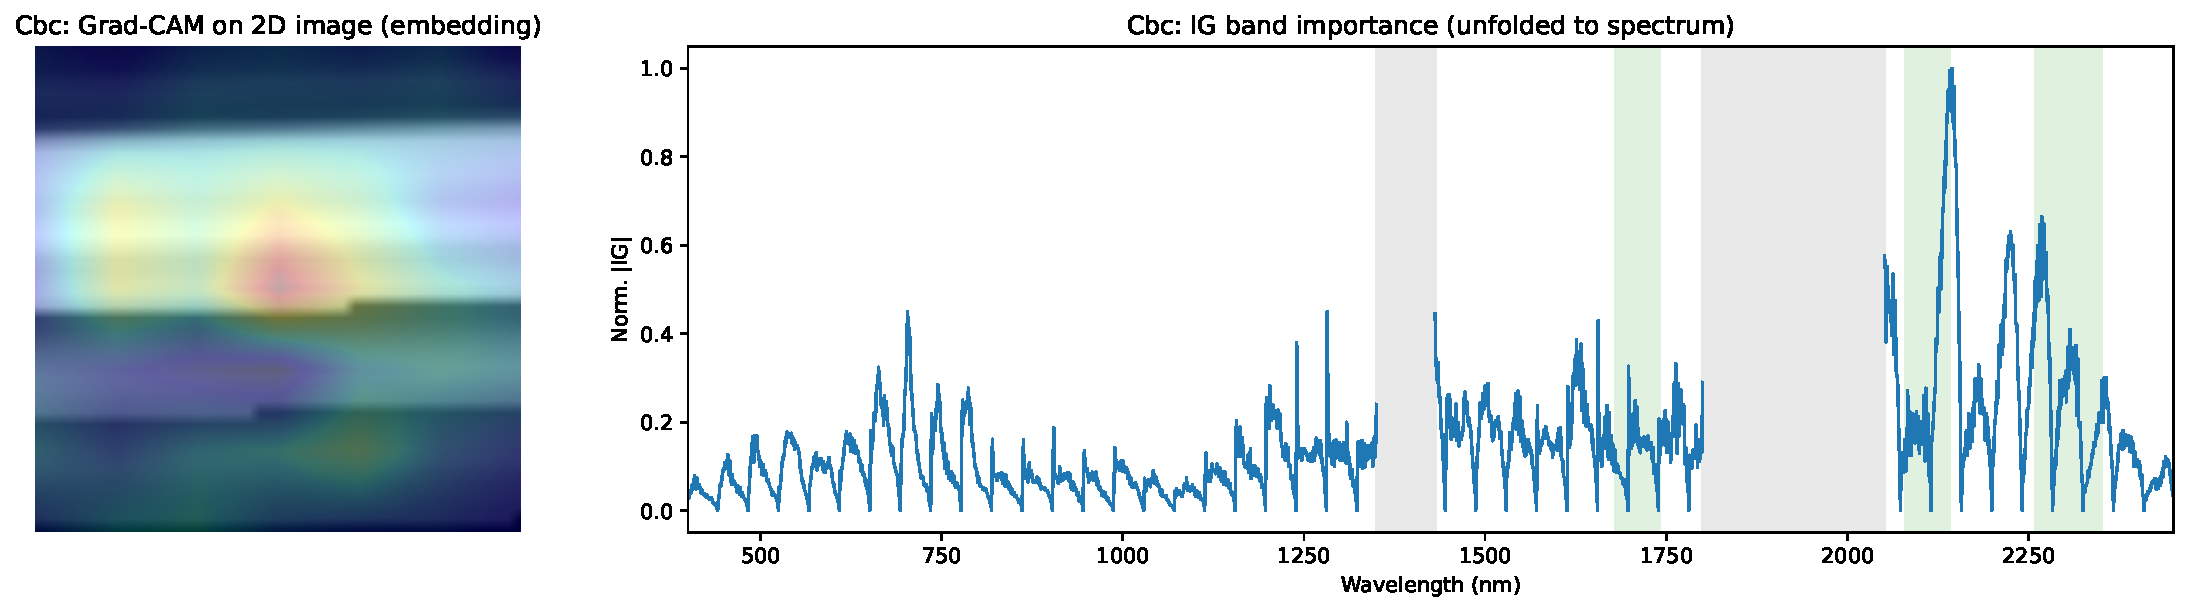
\includegraphics[width=\textwidth]{figures/fig_linking_Cbc.pdf}
    \caption{\jl{Linking 2D and 1D attribution for carbon-based constituents (C\textsubscript{bc}).}}
    \label{fig:linking_cbc}
\end{figure}



% Bibliography settings
%\bibliographystyle{apalike}
%\bibliography{References}

\end{document}
